\documentclass[a4paper, 14pt]{extarticle}

\usepackage{../latexDependencies/misc/preamble2}

\geometry{a4paper}

% Название дисциплины
\newcommand{\subject}{Численные методы} 

% Тип работы
% lab - для лабораторной работы 
% hw  - для домашней     работы
\newcommand{\task}{hw} 

% Номер работы
\newcommand{\taskNumber}{2-3} 

% Название работы
\newcommand{\taskNameOne}{Метод конечных сумм для} 
\newcommand{\taskNameTwo}{интегрального уравнения} 
\newcommand{\taskNameThree}{Фредгольма 2-го рода} 

% Имя студента
\newcommand{\studentName}{Очкин Н.В.}

% Имя преподававателя
\newcommand{\teacherName}{Кутыркин В.А.}

% Группа
\newcommand{\group}{ФН11-52Б}

% Вариант
\newcommand{\variant}{9}

\begin{document}

\graphicspath{ {../latexDependencies/images} } 
\normalsize

\newcommand{\printTask}{%
    \ifthenelse{\equal{\task}{lab}}{%
        лабораторной%
    }{%
        \ifthenelse{\equal{\task}{hw}}{%
            домашней%
        }{%
            Неизвестный тип задания%
        }%
    }%
}

\begin{titlepage}

    \begin{center}
        {\footnotesize \itshape Федеральное государственное бюджетное 
                       образовательное учреждение высшего образования}
    \end{center}

    \begin{minipage}[c]{0.1\textwidth}
        
\includegraphics[width=1.1\textwidth]{iconBMSTU}
    \end{minipage}
    \hfill
    \begin{minipage}[c]{0.9\textwidth}
        \centering
        \itshape
        \bfseries
        \small
        \guillemotleft Московский государственный технический университет \\
        имени Н.Э. Баумана\guillemotright \\
        (национальный исследовательский университет) \\
        (МГТУ им. Н.Э. Баумана) 
    \end{minipage}

    \vspace{0.5cm}
    \noindent\rule{\textwidth}{2pt} \\

    \noindent\uline{\textbf{ФАКУЛЬТЕТ} ФУНДАМЕНТАЛЬНЫЕ НАУКИ} \\
    \vspace{-5pt} \\
    \noindent\uline{\textbf{КАФЕДРА} ВЫЧИСЛИТЕЛЬНАЯ МАТЕМАТИКА И МАТЕМАТИЧЕСКАЯ} \\
    \vspace{-5pt} \\
    \noindent\uline{ФИЗИКА (ФН11)} \\
    \vspace{-5pt} \\
    \noindent\uline{\textbf{НАПРАВЛЕНИЕ ПОДГОТОВКИ} МАТЕМАТИКА И КОМПЬЮТЕРНЫЕ} \\
    \vspace{-5pt} \\
    \noindent\uline{НАУКИ (02.03.01)} \\

    \begin{center}
        \bfseries
        \textsc{О т ч е т} \\[10pt]
        по \printTask {} работе \textnumero {} \taskNumber
    \end{center}

    \vspace{10pt}

    \hspace{10pt} 
    \noindent \textbf{Название \printTask {} работы:} \par
    \vspace{5pt}
    \hspace{10pt} 
    \noindent \textbf{\uline{\taskNameOne}} \vspace{5pt} \\
    \null\hspace{31pt} 
    \textbf{\uline{\taskNameTwo}} \vspace{5pt} \\
    \null\hspace{31pt} 
    \textbf{\uline{\taskNameThree}}

    \vspace{10pt}

    \begin{center}
        \bfseries
        Вариант \textnumero {} \variant
    \end{center}

    \vspace{20pt}

    \hspace{10pt} 
    \noindent \textbf{Дисциплина:} \par
    \vspace{10pt}
    \hspace{10pt} 
    \noindent {\large \subject}

    \vspace{10pt}

    \begin{flushright}
        \renewcommand{\arraystretch}{3}
        \begin{tabular}{r r r}
            \multicolumn{1}{l}{Студент группы \uline{\group}} & 
            $\quad \underset{\text{(Подпись, дата)}}{\underline{\hspace{3cm}}} \quad$ & 
            \multicolumn{1}{c}{$\underset{\text{(И.О. Фамилия)}}{\uline{\textbf{\studentName}}}$} \\

            \multicolumn{1}{l}{Преподаватель} & 
            $\quad \underset{\text{(Подпись, дата)}}{\underline{\hspace{3cm}}} \quad$ & 
            \multicolumn{1}{c}{$\underset{\text{(И.О. Фамилия)}}{\uline{\textbf{\teacherName}}}$} \\
        \end{tabular}
    \end{flushright}

    \vfill

    \begin{center}
        \small
        Москва, 2024
    \end{center}
\end{titlepage}


\newgeometry{left=25mm, right=25mm, top=20mm, bottom=20mm}

\graphicspath{ {../latexDependencies/images/HW2-3} }

% Customize section, subsection, subsubsection and paragraph styles
\titleformat{\section}
  {\normalfont\large\bfseries}{\thesection}{1em}{}

\titleformat{\subsection}
  {\normalfont\normalsize\bfseries}{\thesubsection}{1em}{}

\titleformat{\subsubsection}
  {\normalfont\small\bfseries}{\thesubsubsection}{1em}{}

\titleformat{\paragraph}
  {\small\small\bfseries}{\theparagraph}{1em}{}

% \thispagestyle{empty}

% \null\newpage

% \setcounter{tocdepth}{5}
% \setcounter{secnumdepth}{5}

% \pagenumbering{roman}

% \tableofcontents
% \newpage

% \pagenumbering{arabic}
% \setcounter{page}{1}

\setstretch{1}
\linespread{1.1}

\setlength{\parindent}{0pt}

\fontsize{12pt}{16pt}\selectfont

% \definecolor{myblue}{HTML}{0A88C2}
% \definecolor{myred}{HTML}{FF1B1C}
% \definecolor{mygreen}{HTML}{386641}

% \lstdefinestyle{mystyle}{
%     basicstyle=\ttfamily\footnotesize,
%     keywordstyle=\color{myblue},
%     stringstyle=\color{myred},
%     commentstyle=\color{green!50!black},
%     showstringspaces=false,
%     frame=leftline, 
%     framesep=10pt, 
% }

% % Set the style for Python code
% \lstset{style=mystyle, extendedchars=\true}

% --------------------------------------START--------------------------------------

\section*{Задание}\vspace{-20pt}\rule{\linewidth}{0.1mm}

Используя дискретный аналог уравнения 
\begin{equation*}
    x(s) - \lambda\int\limits^b_a K(s, \tau)x(\tau)d\tau = y(s),\ s \in \left[a; b\right],
\end{equation*}

индуцированный методом конечных сумм с квадратурными формулами прямоугольников
(количество узлов в квадратурной формуле не менее 20), найти приближённое решение
уравнения, которое имеет вид:
\begin{equation*}
    x(s) - \cfrac{1}{n - 47} \cdot \int\limits_0^{\cfrac{N + 7}{N}} 
    K(s, \tau)x(\tau)d\tau = \cfrac{N + 3}{N} \cdot \left(s^2 + \cfrac{n - 53}{2}\right), 
    \quad s \in \left[0; \cfrac{N + 7}{N}\right],
\end{equation*}

где $N$ -- номер фамилии студента в журнале, $n$ -- номер группы и
\begin{equation*}
    K(s, \tau) = \begin{cases*}
        s \cdot \left(2 \cdot \cfrac{N + 7}{N} - \tau \right), \quad 0 \leq s \leq \tau; \\
        \tau \cdot \left(2 \cdot \cfrac{N + 7}{N} - s \right), \quad \tau \leq s \leq. 
        \cfrac{N + 7}{N}
    \end{cases*}
\end{equation*}

Найти аналитическое решение уравнения, сведя интегральное уравнение соответствующей краевой задаче.
В узлах сетки наглядно сравнить приближённое решение с аналитическим, построив
графики этих решений, и оценить абсолютную погрешность приближённого решения.

\section*{Исходные данные}\vspace{-20pt}\rule{\linewidth}{0.1mm}

\begin{equation*}
    n = 52 \qquad N = 9
\end{equation*}

\newpage

\section*{Ход выполнения работы}

\subsection*{Численное решение}\vspace{-20pt}\rule{\linewidth}{0.1mm}

Для построения дискретного аналога, аппроксимирующего уравнение, 
зададим двумерную центрально-равномерную сетку 
$B \times A = \langle(s_i, \tau_i) : s_i \in B, \tau_i \in A \rangle$ 
типа $n \times n$ шага $(h, \tau)$. Следовательно, $B = \langle s_1, s_2, \dots, s_n \rangle$ 
и $A = \langle \tau_1, \tau_2, \dots, \tau_n \rangle$ центрально-равномерные сетки отрезка 
$\left[ a; b \right]$ с шагами $h = \cfrac{b-a}{n}$ и $\tau = \cfrac{b - a}{n}$, 
соответственно.\\

$n$ зададим равным 20, тогда
\begin{equation*}
    n = 20 \qquad \text{отрезок:} \left[ 0; \cfrac{N+7}{N} \approx 1.78 \right]
\end{equation*}
\vspace{-10pt}
\begin{gather*}
    B \hspace{80pt} A \\
    \begin{bmatrix}
        0.088889 \\
        0.17778 \\
        0.26667 \\
        0.35556 \\
        0.44444 \\
        0.53333 \\
        0.62222 \\
        0.71111 \\
        0.8 \\
        0.88889 \\
        0.97778 \\
        1.0667 \\
        1.1556 \\
        1.2444 \\
        1.3333 \\
        1.4222 \\
        1.5111 \\
        1.6 \\
        1.6889 \\
        1.7778
    \end{bmatrix}
    \qquad
    \begin{bmatrix}
        0.088889 \\
        0.17778 \\
        0.26667 \\
        0.35556 \\
        0.44444 \\
        0.53333 \\
        0.62222 \\
        0.71111 \\
        0.8 \\
        0.88889 \\
        0.97778 \\
        1.0667 \\
        1.1556 \\
        1.2444 \\
        1.3333 \\
        1.4222 \\
        1.5111 \\
        1.6 \\
        1.6889 \\
        1.7778
    \end{bmatrix}
\end{gather*}

\newpage

Составим матрицу $K^i_j = K(s_i; \tau_j)$ размера $20 \times 20$:

\begin{center}
    $K^i_j:$ \\[1em]
    \begin{adjustbox}{max width=1\textwidth}
        \renewcommand{\arraystretch}{1}
    $\left[
        \begin{array}{cccccccccccccccccccc}
            0.30815 & 0.30025 & 0.29235 & 0.28444 & 0.27654 & \cdots & 0.16593 & 0.15802 \\
            0.30025 & 0.60049 & 0.58469 & 0.56889 & 0.55309 & \cdots & 0.33185 & 0.31605 \\
            0.29235 & 0.58469 & 0.87704 & 0.85333 & 0.82963 & \cdots & 0.49778 & 0.47407 \\
            0.28444 & 0.56889 & 0.85333 & 1.1378 & 1.1062 & \cdots & 0.6637 & 0.6321 \\
            0.27654 & 0.55309 & 0.82963 & 1.1062 & 1.3827 & \cdots & 0.82963 & 0.79012 \\
            \vdots & \vdots & \vdots & \vdots & \vdots & \ddots & \vdots & \vdots \\
            0.18963 & 0.37926 & 0.56889 & 0.75852 & 0.94815 & \cdots & 2.6548 & 2.5284 \\
            0.18173 & 0.36346 & 0.54519 & 0.72691 & 0.90864 & \cdots & 2.9551 & 2.8207 \\
            0.17383 & 0.34765 & 0.52148 & 0.69531 & 0.86914 & \cdots & 3.1289 & 2.9867 \\
            0.16593 & 0.33185 & 0.49778 & 0.6637 & 0.82963 & \cdots & 3.1526 & 3.0025 \\
            0.15802 & 0.31605 & 0.47407 & 0.6321 & 0.79012 & \cdots & 3.0025 & 3.1605 \\
        \end{array}
    \right]$
    \end{adjustbox}
\end{center}

\vspace{10pt}

Решим СЛАУ:
\begin{equation*}
    \textbf{F} \cdot \upgt x = \upgt y,
\end{equation*}
где \\
$\upgt x = \left[ x^1, \dots, x^n \right>$; \\[1em]
$\upgt y = \left[ y^1, \dots, y^n \right>$; \\[1em]
$\textbf{F} = \left(\delta^i_j - \lambda K^i_j \cdot h \right)^n_n$; \\[1em]
$\lambda = \cfrac{1}{52 - 47} = 0.2$; \\[1em]
$\delta^i_j = \begin{cases*}
    1, \quad i = j; \\
    0, i \neq j.
\end{cases*}$

\begin{center}
    $\textbf{F}:$ \\[1em]
    \begin{adjustbox}{max width=1\textwidth}
        \renewcommand{\arraystretch}{1}
    $\left[
        \begin{array}{cccccccccccccccccccc}
            0.99452 & -0.0053377 & -0.0051973 & -0.0050568 & -0.0049163 & \cdots & -0.0029498 & -0.0028093 \\
            -0.0053377 & 0.98932 & -0.010395 & -0.010114 & -0.0098327 & \cdots & -0.0058996 & -0.0056187 \\
            -0.0051973 & -0.010395 & 0.98441 & -0.01517 & -0.014749 & \cdots & -0.0088494 & -0.008428 \\
            -0.0050568 & -0.010114 & -0.01517 & 0.97977 & -0.019665 & \cdots & -0.011799 & -0.011237 \\
            -0.0049163 & -0.0098327 & -0.014749 & -0.019665 & 0.97542 & \cdots & -0.014749 & -0.014047 \\
            \vdots & \vdots & \vdots & \vdots & \vdots & \ddots & \vdots & \vdots \\
            -0.0033712 & -0.0067424 & -0.010114 & -0.013485 & -0.016856 & \cdots & -0.049444 & -0.051692 \\
            -0.0032307 & -0.0064615 & -0.0096922 & -0.012923 & -0.016154 & \cdots & -0.052534 & -0.050147 \\
            -0.0030903 & -0.0061805 & -0.0092708 & -0.012361 & -0.015451 & \cdots & -0.053096 & -0.050568 \\
            -0.0029498 & -0.0058996 & -0.0088494 & -0.011799 & -0.014749 & \cdots & -0.053377 & 0.94381 \\
        \end{array}
    \right]$
    \end{adjustbox}
\end{center}

\newpage

Составим вектор $\upgt y$:

\begin{equation*}
    \upgt y = \cfrac{N + 3}{N} \left(s^2 + \cfrac{52 - 53}{2} \right) \approx 
    1.33 \left( s^2 - 0.5 \right), \quad s \in \left[ 0; 1.78 \right]
\end{equation*}

\vspace{10pt}

И найдем вектор $\upgt x$:

\begin{equation*}
    \upgt x = \textbf{F}^{-1} \cdot \upgt y
\end{equation*}

\begin{equation*}
    \upgt y: \begin{bmatrix}
        -0.65613 \\
        -0.62453 \\
        -0.57185 \\
        -0.49811 \\
        -0.40329 \\
        -0.28741 \\
        -0.15045 \\
        0.007572 \\
        0.18667 \\
        0.38683 \\
        0.60807 \\
        0.85037 \\
        1.1137 \\
        1.3982 \\
        1.7037 \\
        2.0303 \\
        2.3779 \\
        2.7467 \\
        3.1365 \\
        3.5473 \\
        \end{bmatrix}
    \hspace{50pt}
    \upgt x: \begin{bmatrix}
        -0.50181 \\
        -0.31307 \\
        -0.1015 \\
        0.13171 \\
        0.38526 \\
        0.6577 \\
        0.94753 \\
        1.2531 \\
        1.5727 \\
        1.9045 \\
        2.2467 \\
        2.5974 \\
        2.9545 \\
        3.3161 \\
        3.6801 \\
        4.0445 \\
        4.4073 \\
        4.7664 \\
        5.1197 \\
        5.4654 \\
        \end{bmatrix}
\end{equation*}

\newpage

\subsection*{Аналитическое решение}\vspace{-20pt}\rule{\linewidth}{0.1mm}

Подставляя $K(s, \tau)$ в исходное уравнение, получим:

\begin{equation*}
    x(s) - \cfrac{\int\limits_{0}^{s} \tau \left(\frac{32}{9} - s\right) x(\tau) \, d\tau}{5} - \cfrac{\int\limits_{s}^{\frac{16}{9}} s \left(\frac{32}{9} - \tau\right) x(\tau) \, d\tau}{5} = \cfrac{4 s^{2}}{3} - \cfrac{2}{3}
\end{equation*}

Продифференцируем это уравнение:
\begin{equation*}
    \cfrac{d}{d s} x(s) - \cfrac{\int\limits_{0}^{s} \left(- \tau x(\tau)\right) \, d\tau}{5} - \cfrac{\int\limits_{s}^{\frac{16}{9}} \left(\frac{32}{9} - \tau\right) x(\tau) \, d\tau}{5} = \cfrac{8 s}{3}
\end{equation*} 

Продифференцируем это уравнение во второй раз:
\begin{equation*}
    \cfrac{s x(s)}{5} + \cfrac{\left(\frac{32}{9} - s\right) x(s)}{5} + \cfrac{d^{2}}{d s^{2}} x(s) = \cfrac{8}{3}
\end{equation*}

Упростим выражение:
\begin{equation*}
    \cfrac{32 x(s)}{45} + \cfrac{d^{2}}{d s^{2}} x(s) = \cfrac{8}{3}
\end{equation*}
    
Решая получившееся дифференциальное уравнение, получим:
\begin{equation*}
    x(s) = C_{1} \sin\left(\cfrac{4 \sqrt{10} s}{15}\right) + C_{2} \cos\left(\cfrac{4 \sqrt{10} s}{15}\right) + \cfrac{15}{4}
\end{equation*}

Подставим краевые условия:
\begin{align*}
    x(a) &= x(0) = -\frac{2}{3} \\
    x(b) &= x(1.78) = 0.356 \int\limits_{0}^{\frac{16}{9}} \tau x(\tau) \, d\tau + 3.5473 \\
    x'(b) &= x'(1.78) = 4.741 - 0.2 \int\limits_{0}^{\frac{16}{9}} \tau x(\tau) \, d\tau
\end{align*}

Получим систему краевых условий:
\begin{equation*}
    \begin{cases}
    x(0) = - \cfrac{2}{3} \\[1em]
    0.5625 x\left(\cfrac{16}{9}\right) + \left. \cfrac{d}{d s} x(s) \right|_{\substack{ s=1.78 }} - 1.9954 = 4.7407
    \end{cases}
\end{equation*}
    
Откуда:
\begin{equation*}
    C_1 \approx 1.7535 \qquad C_2 = - \cfrac{53}{12}
\end{equation*}

Итого:
\begin{equation*}
    x(s) = 1.7535 \sin\left(\cfrac{4 \sqrt{10} s}{15}\right) - 4.4167 \cos\left(\cfrac{4 \sqrt{10} s}{15}\right) + 3.75
\end{equation*}

\vspace{10pt}

\subsection*{Анализ результатов}\vspace{-20pt}\rule{\linewidth}{0.1mm}

Построим совмещённые графики аналитически найденной функции $x(s)$ и 
функции, построенной по точкам, найденным численно.

\vfill

\begin{center}
    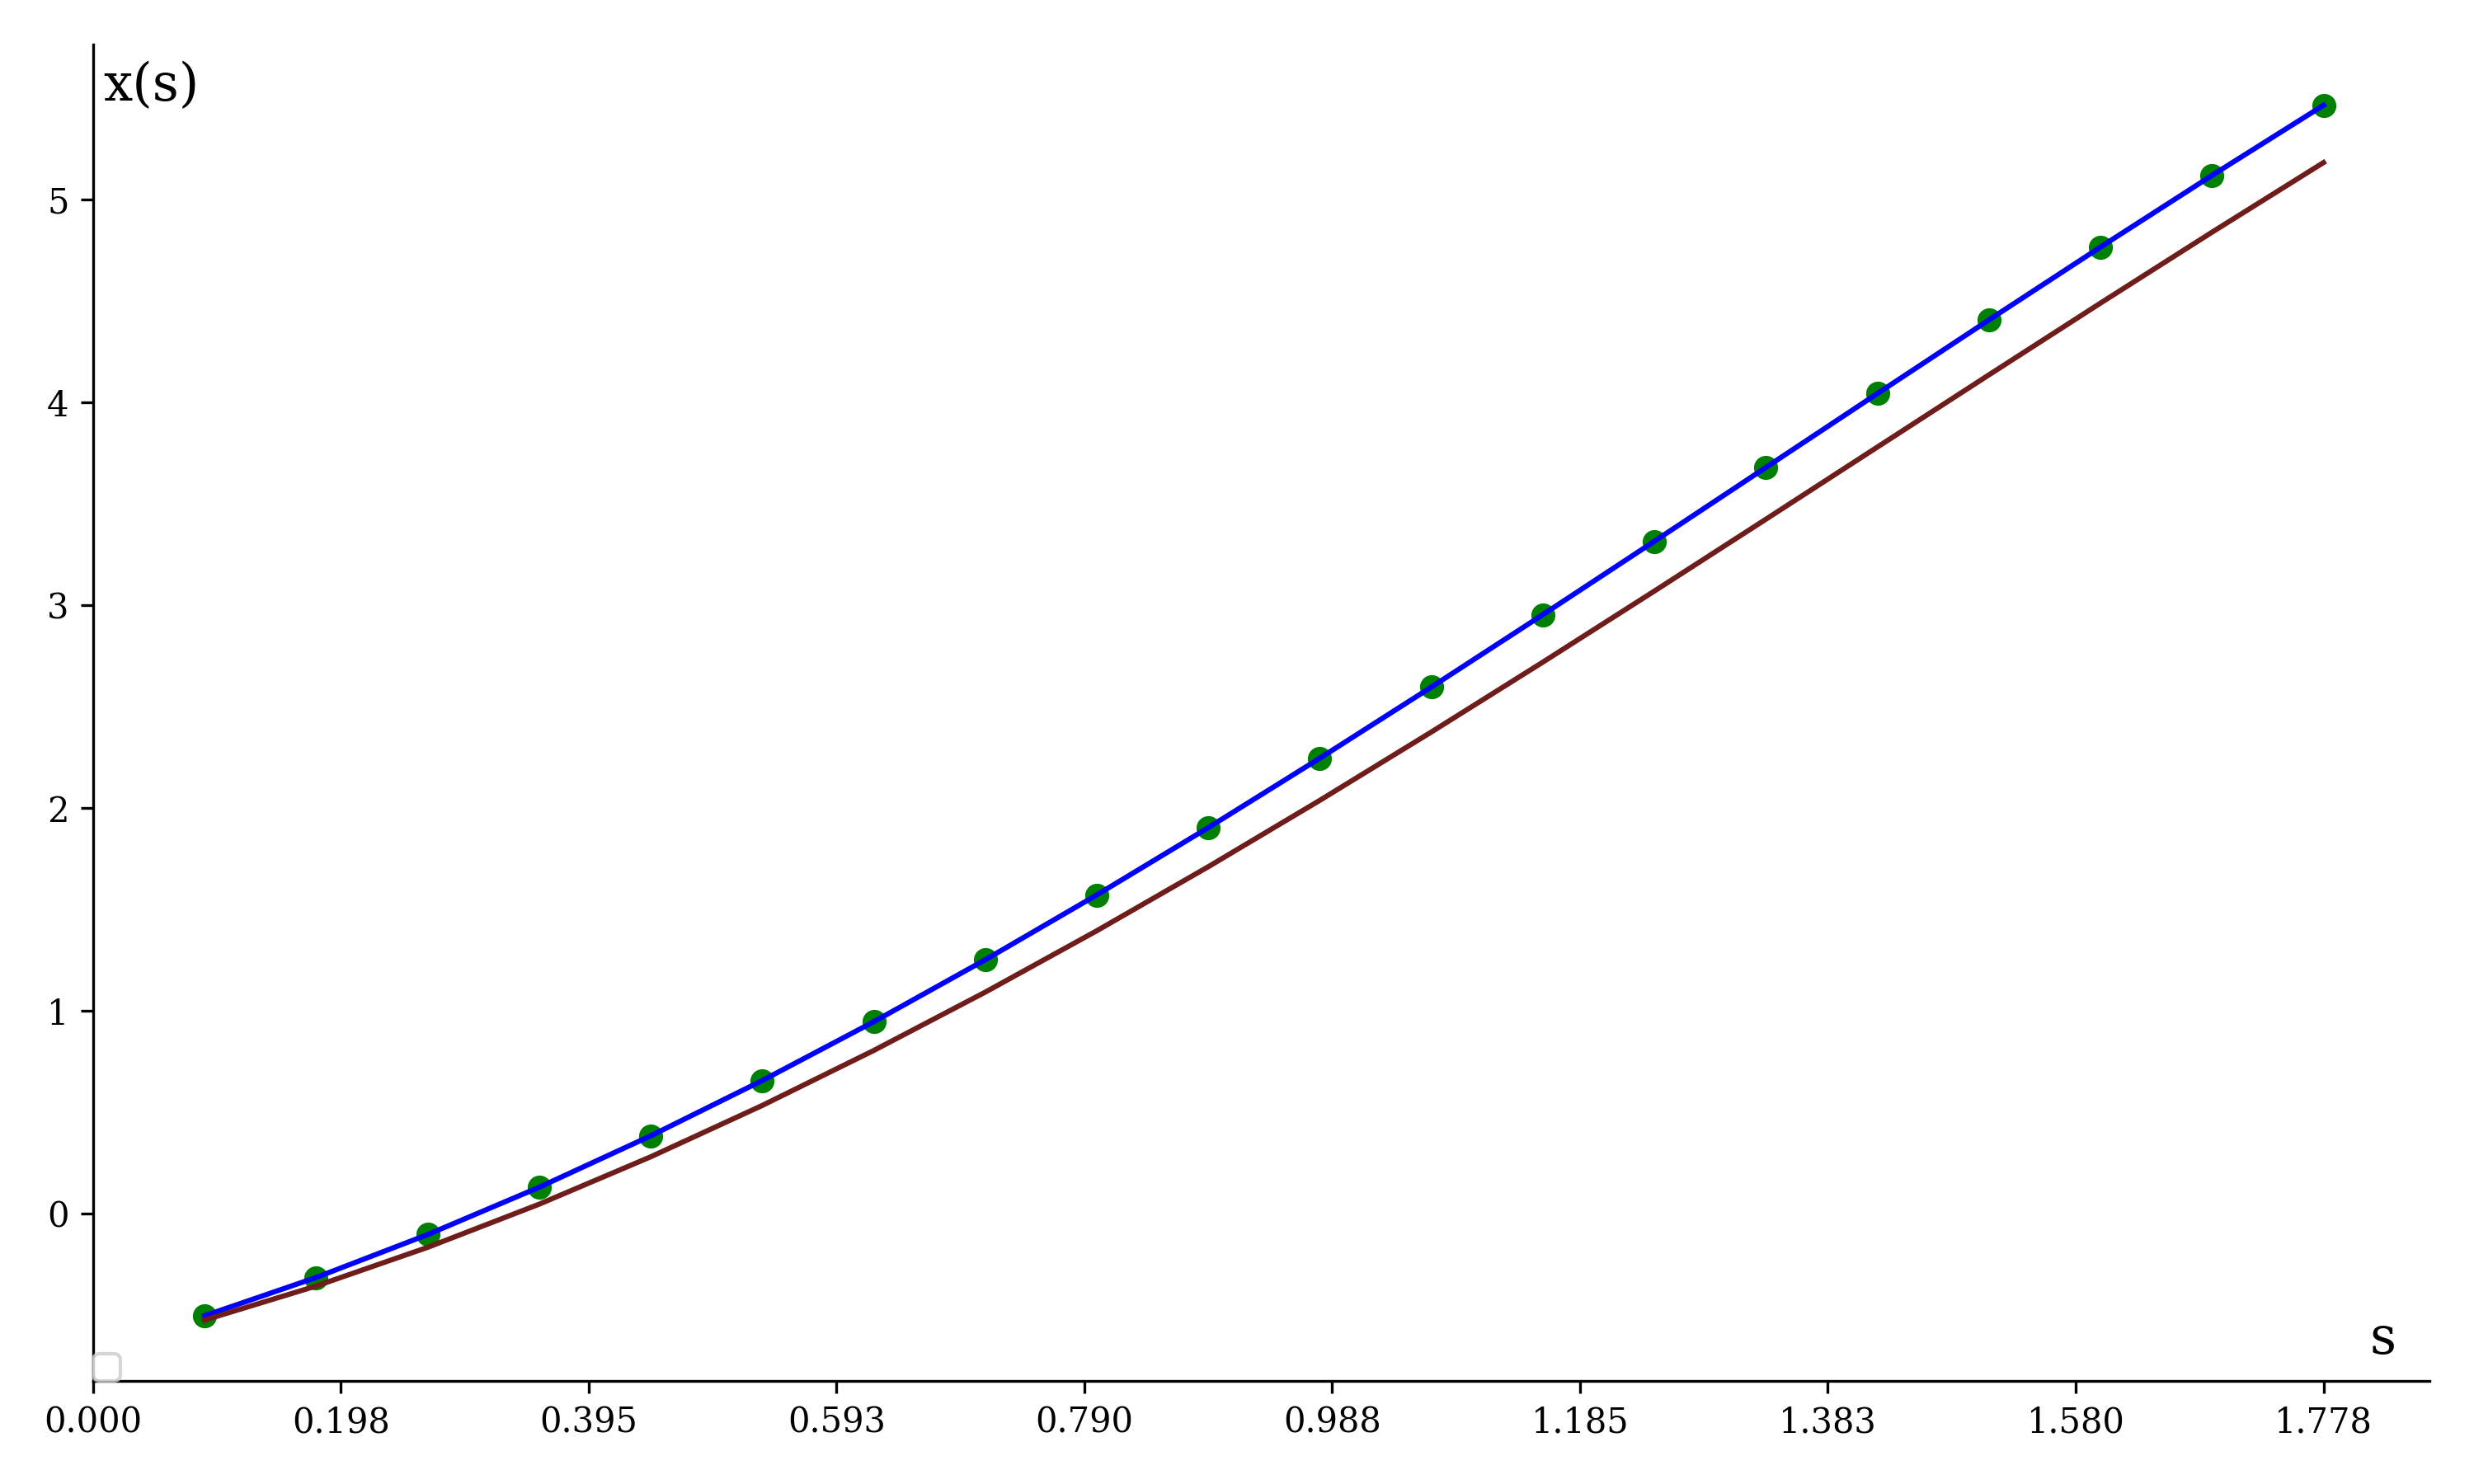
\includegraphics[width=1\textwidth]{plot}
\end{center}

\vfill

\newpage

Вычислим погрешности:

\begin{equation*}
    \setlength{\arraycolsep}{10pt}
    \begin{array}{c c c c}
    s & =x(s) & \approx x(s) & \Delta \\
    \hline
    0.088889 & -0.52295 & -0.50181 & 0.021135 \\
    0.17778 & -0.35523 & -0.31307 & 0.042163 \\
    0.26667 & -0.16446 & -0.1015 & 0.062965 \\
    0.35556 & 0.04829 & 0.13171 & 0.083423 \\
    0.44444 & 0.28183 & 0.38526 & 0.10342 \\
    0.53333 & 0.53485 & 0.6577 & 0.12285 \\
    0.62222 & 0.80593 & 0.94753 & 0.1416 \\
    0.71111 & 1.0935 & 1.2531 & 0.15955 \\
    0.8 & 1.3961 & 1.5727 & 0.17662 \\
    0.88889 & 1.7118 & 1.9045 & 0.1927 \\
    0.97778 & 2.039 & 2.2467 & 0.20771 \\
    1.0667 & 2.3758 & 2.5974 & 0.22155 \\
    1.1556 & 2.7203 & 2.9545 & 0.23415 \\
    1.2444 & 3.0706 & 3.3161 & 0.24544 \\
    1.3333 & 3.4248 & 3.6801 & 0.25535 \\
    1.4222 & 3.7807 & 4.0445 & 0.26383 \\
    1.5111 & 4.1365 & 4.4073 & 0.27082 \\
    1.6 & 4.4901 & 4.7664 & 0.27629 \\
    1.6889 & 4.8395 & 5.1197 & 0.28021 \\
    1.7778 & 5.1829 & 5.4654 & 0.28255 \\
    \end{array}
\end{equation*}
где\\
$=x(s)$ - значение функции в точке, найденной аналитически\\ 
$\approx x(s)$ - значение функции в точке, найденной численно\\ 
$\Delta$ - абсолютная погрешность 

\begin{equation*}
    \text{max} \Delta: \hspace{3pt} 0.28255
\end{equation*}

\subsection*{Вывод}\vspace{-20pt}\rule{\linewidth}{0.1mm}

В ходе проделанной работы было решено интегральное уравнение Фредгольма 
второго рода с симметричным, непрерывным и аналитически заданным ядром 
методом конечных сумм, найдено его аналитическое решение и сравнены результаты 
обоих вычислений.

\end{document}
